\documentclass[10pt,letterpaper,notumble]{leaflet}
\usepackage[T1]{fontenc}
\usepackage[utf8]{inputenc}
\usepackage{listingsutf8}
\usepackage[spanish]{babel}
\usepackage{microtype}
\usepackage{blindtext} 
\usepackage{biolinum} 
\renewcommand\rmdefault{\sfdefault}% Verwende serifenlose Schrift 
\usepackage{mwe}% Dummy Bilder 
\usepackage{graphicx}
\usepackage{verbatim}
\usepackage{xcolor}
	\definecolor{WildStrawberry}{rgb}{1.0, 0.26, 0.64}
	\definecolor{wildstrawberry}{rgb}{1.0, 0.26, 0.64}
	\definecolor{Mulberry}{rgb}{0.77, 0.29, 0.55}
	\definecolor{LimeGreen}{rgb}{0.2, 0.8, 0.2}
	\definecolor{LincolnGreen}{rgb}{0.11, 0.35, 0.02}
	\definecolor{blue}{rgb}{0.0, 0.0, 1.0}
	\definecolor{forestgreen(traditional)}{rgb}{0.0, 0.27, 0.13}
\usepackage[colorlinks,citecolor=blue,urlcolor=blue]{hyperref}


\AddToBackground{5}{\put(0,0){\textcolor{blue!5}{\rule{\paperwidth}{\paperheight}}}}%

\AddToBackground{5}{% Fondo de la página pequeña 1
	\put(\LenToUnit{0.05\paperwidth},\LenToUnit{0.875\paperheight}){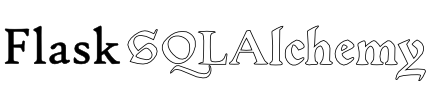
\includegraphics[width=\LenToUnit{0.90\paperwidth},height=\LenToUnit{0.1\paperheight}]{../img/flask-sqlalchemy-title.png}}
}

\title{Quik Reference} 
\author{Ferreira Juan David} 
\date{\today} % Experiment 1
\AddToBackground{4}{\put(0,0){\textcolor{blue!5}{\rule{\paperwidth}{\paperheight}}}}%

\begin{document}
    Pero aún no están en la base de datos, así que asegurémonos de que estén:
    {\footnotesize
    \begin{verbatim}
>>> db.session.add(admin)
>>> db.session.add(guest)
>>> db.session.commit()
    \end{verbatim}}
    
    \vspace*{-0.3cm}
    
    Acceder a los datos en la base de datos es muy fácil:
    
    \vspace*{-0.3cm}
    
    {\footnotesize
    \begin{verbatim}
>>> User.query.all()
[<User u'admin'>, <User u'guest'>]
>>> User.query.filter_by(username='admin').first()
<User u'admin'>
    \end{verbatim}}

    \vspace*{-0.3cm}
    
    Observemos que nunca hemos definido un método \texttt{\_\_init\_\_} en la clase \texttt{User}. Esto es porque \texttt{SQLAlchemy} agrega un constructor implícito a todas las clases del modelo que acepta argumentos de palabras clave para todas sus columnas y relaciones. Si decidimos anular el constructor por cualquier motivo, debemos asegurarnos de seguir aceptando \texttt{**kwargs} y llamar al superconstructor con esos \texttt{**kwargs} para preservar este comportamiento:
    
    \vspace{5cm}
    
     \lstset{
    	inputencoding=utf8/latin1,
    	basicstyle=\footnotesize\ttfamily,
    	commentstyle=\color{LincolnGreen},
    	frame=lines,
%    	frame=single,
    	language=python,
    	label={lst:code_direct},
%    	numbers=left,
%    	numbersep=10pt,
%    	numberstyle=\footnotesize\color{gray},
    	showstringspaces=false,
    	stringstyle=\color{Mulberry},
    	%                	otabsize=3,
    	% the more interesting/new bits
    	classoffset=1,% starting a new class
    	morekeywords={True},
    	keywordstyle=\color{WildStrawberry},
    	classoffset=2,% starting another class
    	morekeywords={False},
    	keywordstyle=\color{blue},
    	classoffset=0,% restore to default class if more customisations...
    	morekeywords={self, class, def},
    	keywordstyle=\color{LimeGreen},
    	classoffset=2,% starting another class	
    }
    \lstinputlisting[language=Python,
    firstline=17,
    lastline=21]{../python/01-quick-start.py}
    
    \section{Relaciones simples}
    
    \texttt{SQLAlchemy} se conecta a bases de datos relacionales y estas son realmente buenas para establecer relaciones. Como tal, tendremos un ejemplo de una aplicación que usa dos tablas que tienen una relación entre sí:
    
    \thispagestyle{empty}% Keine Seitenzahlen 
    
    \makebox[\linewidth][l]{
    	\begin{minipage}{2.2\linewidth}
                
                \lstinputlisting[language=Python,
                                 firstline=23,
                                 lastline=46]{../python/01-quick-start.py}
                                 
                Primero creemos algunos objetos:
               	
                \lstinputlisting[language=Python,
                firstline=48,
                lastline=52]{../python/01-quick-start.py}
                
                Como podemos ver, no es necesario agregar los objetos \texttt{Post} a la sesión. Dado que \texttt{Category} es parte de la sesión, también se agregarán todos los objetos asociados a él a través de relaciones. No importa si \texttt{db.session.add()} se llama antes o después de crear estos objetos. La asociación también se puede hacer en cualquier lado de la relación, por lo que se puede crear una publicación con una categoría o se puede agregar a la lista de publicaciones de la categoría.
                
                Veamos las publicaciones. Acceder a ellos los cargará desde la base de datos, ya que la relación se carga de forma diferida, pero probablemente no notaremos la diferencia: cargar una lista es bastante rápido:
                
                \lstinputlisting[language=Python, firstline=54, lastline=55]{../python/01-quick-start.py}
                
                Si bien la carga diferida de una relación es rápida, puede convertirse fácilmente en un cuello de botella importante cuando se generan consultas adicionales en un bucle para más de unos pocos objetos. Para este caso, \texttt{SQLAlchemy} nos permite anular la estrategia de carga en el nivel de la consulta. Si deseamos que una sola consulta cargue todas las categorías y sus publicaciones, podemos hacerlo así:
                
                \lstinputlisting[language=Python, firstline=57, lastline=61]{../python/01-quick-start.py}
                
                Si deseamos obtener un objeto de consulta para esa relación, podemos hacerlo usando \texttt{with\_parent()}. Excluyamos esa publicación sobre \texttt{Snakes}, por ejemplo:
                
                \lstinputlisting[language=Python, firstline=63, lastline=64]{../python/01-quick-start.py}
            
        \end{minipage}
    
    }
    \clearpage % end the column
    \mbox{}
    \clearpage
    
    \section{Camino a la iluminación}
    
    Lo único que necesita saber con respecto a \texttt{SQLAlchemy} es que:
    
    \begin{enumerate}
    	\item \texttt{SQLAlchemy} le da acceso a las siguientes cosas:
    	
    	    \begin{itemize}
    	    	\item[$\bullet$] Todas las funciones y clases de \texttt{sqlalchemy} y \texttt{sqlalchemy.orm}.
    	    	
    	    	\item[$\bullet$] Una sesión de ámbito preconfigurada llamada \texttt{session}.
    	    	
    	    	\item[$\bullet$] La \texttt{metadata} y la \texttt{engine}.
    	    	
    	    	\item[$\bullet$] Los métodos \texttt{SQLAlchemy.create\_all()} y \texttt{SQLAlchemy.drop\_all()} para crear y eliminar tablas según los modelos.
    	    	
    	    	\item[$\bullet$] Una clase \texttt{Model} base que es una base declarativa configurada.
    	    \end{itemize}
    	
    	\item La clase \texttt{Model} base declarativa se comporta como una clase \texttt{Python} normal, pero tiene un atributo \texttt{query} adjunto que se puede usar para consultar el modelo. ( \texttt{Model} y \texttt{BaseQuery})
    	
    	\item Tiene que confirmar la sesión, pero no tiene que eliminarla al final de la solicitud, \texttt{Flask-SQLAlchemy} lo hace por usted
    \end{enumerate}
    
    \clearpage % end the spanned column
    
    \maketitle
    \begin{abstract}
    	\href{https://flask-sqlalchemy.palletsprojects.com/en/2.x/#requirements}{\texttt{Flask-SQLAlchemy}} es una extensión para \href{https://flask.palletsprojects.com/en/1.1.x/}{\texttt{Flask}} que agrega soporte para \href{https://www.sqlalchemy.org/}{\texttt{SQLAlchemy}} a nuestras aplicaciones. Su objetivo es simplificar el uso de \texttt{SQLAlchemy} con \texttt{Flask} proporcionando valores predeterminados útiles y helpers adicionales que facilitan la realización de tareas comunes.
    	
    	Consulte la documentación de \texttt{SQLAlchemy} para aprender a trabajar con el \texttt{ORM} en profundidad. La siguiente documentación es una breve descripción general de las tareas más comunes, así como de las características específicas de \texttt{Flask-SQLAlchemy}.
    \end{abstract}
    \begin{center}
    	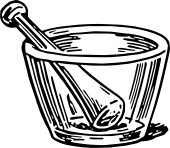
\includegraphics[width=\textwidth]{../img/flask-sqlalchemy-logo.png}
    \end{center}

    \thispagestyle{empty}
    
    \clearpage
    
    \section{Requisitos}
    
    \begin{tabular}{||c||c||c||c||}
    	\hline
    	\hline
    	\rule[-1ex]{0pt}{2.5ex} Our Version & Python & Flask & SQLAlchemy \\
    	\hline
    	\rule[-1ex]{0pt}{2.5ex} 2.x & 2.7, 3.4+ & 0.12+ &
    	\begin{minipage}[c]{0.25\textwidth}
    		\vspace{0.2cm}
    		\footnotesize{0.8+ or 1.0.10+}
    		
    		w/Python 3.7
    	\end{minipage}
    	 \\
    	\hline
    	\rule[-1ex]{0pt}{2.5ex} 3.0+ (in dev) & 2.7, 3.5+ & 1.0+ & 1.0+ \\
    	\hline
    	\hline
    \end{tabular}
    
    \section{Guía de Usuario}
    
    \subsection{Inicio rápido}
    
    \texttt{Flask-SQLAlchemy} es fácil de usar en aplicaciones básicas y se escala fácilmente para aplicaciones más grandes. Para obtener la guía completa, consulte la documentación de la \texttt{API} en la clase \href{https://flask-sqlalchemy.palletsprojects.com/en/2.x/api/#flask_sqlalchemy.SQLAlchemy}{\texttt{SQLAlchemy}}.
    
    Una vez instanciado, este objeto contiene todas las ``\texttt{funciones}'' y ``\texttt{helpers}'' de \texttt{sqlalchemy} y \texttt{sqlalchemy.orm}. Además, proporciona una clase llamada \texttt{Model}, que es una base declarativa que se puede usar para declarar modelos:
    
    \lstinputlisting[language=Python,
                     firstline=1,
                     lastline=15]{../python/01-quick-start.py}
    
    Para crear la base de datos, importamos el objeto \texttt{db} desde un shell de \texttt{Python} o de \texttt{Flask}
    \vspace*{-0.3cm}
    
    {\footnotesize
    \begin{verbatim}
(venv) D:\Documents\venv\Flask\sqlalchemy> flask shell
    \end{verbatim}}
    
    \vspace*{-0.4cm}
    
    y ejecutamos el método \texttt{SQLAlchemy.create\_all()} para crear la base de datos y sus tablas:
    
    \vspace*{-0.4cm}
    
    {\footnotesize
    \begin{verbatim}
>>> from app import db
>>> db.create_all()
    \end{verbatim}}

    \vspace*{-0.4cm}
    
    Lo que crea nuestra base de datos. Ahora para crear algunos usuarios
    
    \vspace*{-0.3cm}
    
    {\footnotesize
    \begin{verbatim}
>>> from app import User
>>> admin = User(username='admin', email='admin@xyz.com')
>>> guest = User(username='guest', email='guest@xyz.com')
    \end{verbatim}}

\end{document}